\documentclass[11pt]{article}
\setlength\parindent{0 in}
\setlength\parskip{0.1 in}
\usepackage{fullpage}
\usepackage{amsmath}
\usepackage{graphicx}

\begin{document}
\title{Making an FPGA-based Digital Down-Converter: Ay121 Lab Instructions}

\maketitle

For the next two weeks, we'll be exploring real-time digital signal 
processing with state-of-the-art digital computing hardware.  We're going
to use a ROACH board designed by the Collaboration for Astronomy Signal
Processing and Electronics Research (CASPER).  This board employs a
massively parallel Field-Programmable Gate Array processor, and could,
with the exception of a front-end amplifier, possible replace the entire
wall of hardware in the radio lab.  

In this lab, we're going to replace only a part of that hardware; we'll
turn the ROACH into a digital mixer and filter (which we together will
call a down-converter).  Each {\it group} will work together on programming
the ROACH board using the Simulink programming language.  Once a design
is compiled, each group will setup a noise test on the bench with the ROACH
running their compiled design.  However, each {\it individual} will choose
her own coefficients to use in the FIR filter we implement.  Each individual
will then record her own filtered and unfiltered data, and use this data
to measure the per-frequency response of her filter coefficients.  The individual
will compare this measured response to the analytic response she predicts through
analysis in IDL.

% ---------------------------------------------------------------------------
\section{Accessing Simulink}

\subsection{Setting up a VNC Session}

From any *nix computer:
\begin{verbatim}
$ ssh username@host.computer.edu
    (enter password)
$ vncserver
    (write down XX of "desktop is host.computer.edu:XX)
$ exit
\end{verbatim}
This will set up a VNC session for you to log into in the future.  Remember
your session number (XX).

When you are done with your session, it would be neighborly of you to free up the computer resources associated with your vnc session:
\begin{verbatim}
$ ssh username@host.computer.edu
$ vncserver -kill :XX
    (where XX is your VNC session from above)
$ exit
\end{verbatim}
Thanks!


\subsection{Accessing Your VNC Session}

From any *nix computer:
\begin{verbatim}
$ vncviewer -via username@host.computer.edu localhost:XX
    (ssh password)
    (vnc password)
\end{verbatim}

All future commands are to be typed inside your VNC session.

\subsection{About Simulink on Linux}

The machine you are logged into is running a Linux desktop.
It behaves somewhat differently than other desktop environments you may be
used to.  Because Simulink sometimes opens windows that are larger than
the size of the desktop, it may be useful to know that you can move these
windows around by right-clicking, selecting "Move", and then dragging the window around.

\subsection{Starting Matlab/Simulink}

Make sure there is a file "startup.m" in your directory.  If it does not
exist, copy it there from /opt/casper/startup.m.  This file is required to
automatically load some signal processing libraries when you start up
the design tools.  To start Matlab/Simulink, type:

\begin{verbatim}
$ simmy
\end{verbatim}

This program is a script that sets up the licenses for all the tools we'll be
using, and then executes the program ``matlab''. 

\section{Introduction to Simulink and ROACH}

We have a tutorial at http://casper.berkeley.edu/astrobaki/index.php/CasperTutorial01
that will run you through the basics of FPGA design with Simulink.  Skip section 8 of
the tutorial--it runs through some software (KATCP) that you won't need use.

A few details from that tutorial are different for the setup in our lab.  For one, 
the ROACH we use has an "lx110t" FPGA, which is different from the "sx95t" that is
selected in the {\it XSG Core Config} block in the tutorial. 
Our ROACH in the lab is at IP address 10.32.92.113, but can also be called "roach".  
Whenever you get to the part about
sending your *.bof file over to the ROACH, you'll need to first scp the file to 
your account in the lab, and then copy the file from there to root@roach:/boffiles.
To read/write from the registers in your design, you an ssh in from any computer in the lab,
but for an authentic experience, you might want to ssh in from a computer on the bench.
That way, you can see die blinken lichten, and you won't have the problem of two people
trying to program the FPGA at the same time.

Here are a couple other pointers that weren't in the tutorial:
\begin{itemize}
\item In the window containing your Simulink design, choose {\it Format $\rightarrow$ 
Port/Signal Displays $\rightarrow$ Port Data Types}.  Although this will complain
if your design isn't complete (i.e. if there are errors), it will tell you the data
type of each wire of a working design.  This can really help you follow how your
design works and catch bugs before compiling.  If you change your design, hit Ctrl-D
to update the labels.
\end{itemize}

\section{Capturing ADC Samples}

Now that you are more-or-less familiar with the Simulink programming language, it's
time to create a design that captures raw data samples from the Analog-to-Digital
Converter attached to the ROACH.

\subsection{The Simulink Design}

The ADC we are using is a Quad-ADC or "quadc", so named because it actually digitizes
4 independent signals.  We'll only be using one signal.  To interface to the QADC, drag in a
{\bf quadc} yellow block from the BEE\_XPS System Blockset.  Providing appropriate simulation inputs,
connect the "data0" output line to a {\bf Shared BRAM}, and rename that BRAM to "data\_bram".
Configure the Block RAM (BRAM) to hold a lot (at least 2048) data samples.  

Next, you'll want to
create a mechanism for triggering a capture of data into the Shared BRAM.  This circuit should walk
through all of the addresses in the BRAM sequentially, writing a new ADC sample into each slot.  
Once the last address is reached, the counter should halt, and data should stop being written.  The
system should then wait until you reconfigure a {\bf Software Register} (renamed to "trig") to
trigger a new data capture.

\begin{figure}
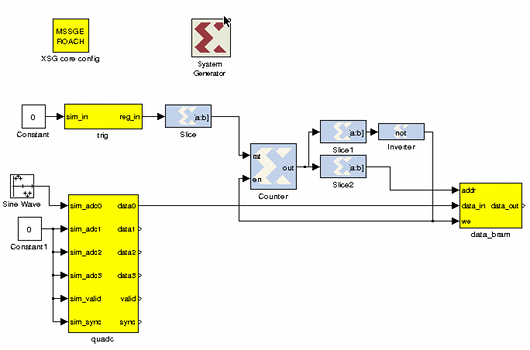
\includegraphics[width=4in]{adc_capture.png}
\end{figure}

A picture of a working design has been included as a reference should you get stuck.  However, you'll
have to figure out the block parameters for yourself.  One thing to be sure of: make sure the {\bf XSG Core Config}
block in your design is set for "User IP Clock Source" = "adc0\_clk".  This uses the ADC sample clock 
to clock the FPGA, so everything marches through the FPGA at the rate that samples arrive.

Remember to simulate your design to ensure everything is working before you compile!

\subsection{Running the Design}

After compiling, transfer the *.bof file over to the ROACH as before, and run it.  Make sure the sample clock
to the ADC is set to 200 MHz, and is on before you program the FPGA.  FPGAs behave very erratically if they aren't
clocked properly; if you program the FPGA and then turn on the clock, you may see gibberish, or even nearly-correct
behavior that occasionally goes whacky.  Also check that you have attached a 
noise signal into the ADC, so that you get something interesting in your BRAM.  You can now write appropriate 
values to "trig" to initiate a data capture.  You can use hd to look at values in "data\_bram" and make sure things
make sense.  When you are happy with the contents of the BRAM, use your account at the lab to scp the contents of the
BRAM to a computer with IDL:
\begin{verbatim}
$ scp root@roach:/proc/PID/hw/ioreg/data_bram .
\end{verbatim}

Create a power spectrum of the noise you recorded, with a number of channels at least a factor of 8 smaller than
the number of ADC samples you captured.  Use the fact that you can compute several such power spectra over the 
window of samples you aquired to beat down the noise in your measurement of the noise power spectrum. 
\begin{enumerate}
\item Plot the power spectrum of the noise you recorded, integrated over multiple DFT windows
\end{enumerate}
You might be noticing a huge spike of power in the frequency 0 bin.  This comes from a voltage bias at the input
of the ADC.  The specification for this ADC allows for up to 3 bits of signal bias.  You'll probably want to 
zero out this bin to make your plots look better. Remember to omit this bin from your coming analysis.

\section{Applying a Summing Filter}

Modify (but save to a new file) your design to capture ADC samples, so that two adjacent input time samples are summed
to produce each output sample.  States more precisely, produce the output $S$ such that:
\begin{equation}
S_i = X_{i-1} + X_{i-2}
\end{equation}
where $X_i$ are input samples.  The latency of your summing filter is unimportant.

Before programming the ROACH with this design:
\begin{enumerate}
\item Can you predict a priori what frequency response this time-domain 
summing filter will produce (hint: it {\it is} an analytic function)?
\item If you don't know yet what the response function will be, simulate it with noise in IDL 
to obtain a low-noise predicted filter response (in units of power).  If you do know the response, 
generate the exact filter response.
\end{enumerate}

Follow the same steps you used for the ADC capture design, inject the same noise source and
capture a new set of time domain samples drawn from after the application of the summing filter.
\begin{enumerate}
\item Plot the power spectrum of the filtered noise you recorded, integrated over multiple DFT windows
\end{enumerate}

You now have two sets of time-domain samples, each drawn from the same noise source and digitized with the same
ADC, but one has had a digital filter applied.  Given that the noise source and the ADC do not have a perfectly
flat response versus frequency:
\begin{enumerate}
\item Use your measured power spectra to isolate the inherent response of your summing filter
\item Overlay on your measured filter response the filter response you predicted
\item Is your prediction accurate to within the noise of your measurements? What are your error bars?
\end{enumerate}

\section{Create an FIR Filter}

Implement an 8-tap FIR filter:
\begin{equation}
S_i = \sum_{n=0}^7{C_nX_{i-n}}
\end{equation}
The coefficients of this filter, $C(t)$, will be a function that convolves the input signal, $X(t)$, to produce the time-domain filtered response $S(t)$:
\begin{equation}
S(t) = C(t)\ast X(t)
\end{equation}
Since a convolution in time-domain is multiplication in the frequency domain,
this convolution is equivalent to:
\begin{equation}
\hat S(\omega) = \hat C(\omega)\cdot\hat X(\omega)
\end{equation}

You will want to implement the FIR coefficients with run-time programmable with {\bf Software Registers}.  You may find it useful in Simulink to
highlight a set of blocks and right-click $\rightarrow$ {\it Create Subsystem}.  This will create a block that
you can rename, copy, and paste just as any other block, but underneath contains your blocks.  You can open it
by double-clicking.  A stylistic point: I recommend against putting yellow blocks in subsystems (although I do
break this rule sometimes).  The rationale is that once you compile your design, you'll want to know at a 
glance what the interfaces are.  If you hide your interfaces in subsystems, it's hard for a user to see quickly how
they are supposed to interact with the design.

Copy your previous design for capturing time-domain samples.  Before programming the ROACH with this design:
\begin{enumerate}
\item Choose coefficients that implement a 5/8-band filter (a filter that, if you divided the band into 8 complex
channels, would extract the 5 channels centered around 0):
\subitem Choose the frequency-domain response you want for your filter (i.e. the function you would like to multiply
the frequency spectrum of your noise by to "filter" it)
\subitem Compute the real-valued, time-domain coefficients that implement that filter, keeping in mind that: 
\subsubitem Multiplication in the frequency domain is a convolution in the time domain
\subsubitem The Fourier transform of a real-valued signal has the property that:
$\hat f(\omega) = \hat f^*(-\omega)$
\subsubitem You will want to think carefully about where the 0 frequency bin is
\subsubitem The FFT puts negative frequencies after positive frequencies in your array.  Similarly, when you take the inverse, it will put negative times after positive times.  When implementing your coefficients in an FIR, though, negative times {\it have} to operate on samples that arrive before positive times.
\item In what order are you going to write these coefficient into the software registers of your FIR filter?
\item Plot the predicted filter response for your coefficients at a frequency resolution much finer than an 8-channel
DFT produces.  The best way to do this will be to add more time-domain samples to your coefficients.  We don't want to introduce any new signal, though, so just add zeros to pad your coefficients out to 64 samples, and then transform the result back into the time domain.  
\item Why aren't the passband and stopband flat?
\end{enumerate}

Now collect data from the noise source, filtered through the FIR filter programmed with your coefficients.  As before:
\begin{enumerate}
\item Isolate the inherent response of your FIR filter
\item Compare your measured filter response to filter response you predicted
\item Is there a way you can think of to create the exact same FIR filter (which has symmetric positive and negative
frequency response) using half the number of multipliers and software registers?  There's no need to actually do it,
unless you want to.
\end{enumerate}

\section{Add a Mixer}

As a final touch, we'll add a digital mixer.  Compared to an FIR filter, this will be pretty quick.  The only trick
is creating a digital sine and cosine.  We'll take the easy way out here, and use the {\bf SineCosine} block from the
{\it Xilinx Blockset $\rightarrow$ Math} library.  The "theta" input should just be a counter.  The number of bits
in the counter will determine the period of the sine/cosine wave generated.  Although it looks fancy, it's really just
a BRAM loaded with coefficients, and "theta" is the address.  For a reason I'm not privy to, the "theta" port must be
at least 3 bits.  If you want something that cycles faster than a 3-bit counter, you'll have to concatenate a counter
and zeros to pad the signal out to 3 bits.

\begin{enumerate}
\item If you will be clocking this design at 200 MHz, and you want to mix 
at 50 MHz, what should the sample period of your sine/cosine be?
\end{enumerate}

Mixing with a sine/cosine gives you In-phase and Quadrature signals, which we'll take to be a complex number.
Our FIR filter was only equipped to handle real numbers.  Fortunately, extending the FIR filter for complex numbers
should really just be a matter of copy-paste, especially if you kept your coefficient registers on the top level.  We
would like to keep just one set of coefficients to avoid unnecessary interfaces.  You'll also notice that we
need to rework the {\bf Shared BRAM} block, since we now have real and imaginary components to record.  You can
either:
\begin{itemize}
\item cop out and add a second bram that attaches to the same address and write-enable so that it records data at the
{\it exact} same time as the other one, or
\item keep your design slim by trimming and concatenating the signal to fit into the 32-bit data\_in port.  If you go
this route, pay attention to your data types and don't forget to make your Shared BRAM of unsigned data type.
\end{itemize}

A major challenge in creating an analog down-converter lies in creating sine/cosine waves that are perfectly in
phase with one another, and in carefully matching the filters on the real and imaginary components of the mixer product.
Any mismatch in phase or response creates an "mirroring" problem, whereby a positive frequency will have a small
mirror image at the corresponding negative frequency.  Perfectly in-phase sine/cosine signals and perfectly matched
filters come for free in our digital down-converter.  This is nothing to sneeze at.  Digital down-converters have only
recently become viable at radio frequencies, and they are fast supplanting their analog forebearers.

Finally, let's prove the down converter works.  Create a new signal input that is the sum of noise and a 60 MHz sine wave.
Record the down-converted result, and:
\begin{enumerate}
\item Plot the time-averaged power spectrum of the signal.
\item At what frequency should the output tone be?  How many samples the period of this tone?
\item What is the range (in MHz) of the passband of your FIR filter?
\item Through your FIR filter, the number of bits increased with each operation.  Why was it okay, for those who
fit the complex data into one Shared BRAM output, to reduce the number of bits?  What would be the minimum number of
bits you need to output the signal without significant loss in precision?
\item If you knew that the signal you were processing was noise-dominated, and your FIR filter's coefficients were
set to quarter the bandwidth, could you shave any more off the minimum number of bits needed in your complex number?
Explain.
\end{enumerate}

\section{Conclusion}

Hopefully you've gotten a taste for how digital signal processing works on an FPGA.  Simulink is a fun graphical
programming tool that captures the inherently parallel nature of circuit design.  Programming for parallel processing
is a lot different than the iterative processing model we are used to thinking about when programming CPUs.  If
you enjoy the challenge of programming FPGAs and are thirsty for more, the CASPER group supports undergraduate
research in the field of radio astronomy instrumentation and digital signal processing.  Many of 
us use FPGA programming and instrument design as tools for furthering our science objectives in 
radio astronomy, and welcome interested students.  Feel free to contact Aaron Parsons (aparsons@astron) for more
information.

\end{document}